\documentclass[00-GLMregslides.tex]{subfiles}
\begin{document}
	%================================================ %
	\begin{frame}[fragile]
		\frametitle{Negative Binomial Regression with \texttt{R} }
		\large
		
		\begin{framed}
			\begin{verbatim}
			
				newdata1 <- data.frame(math = mean(dat$math), prog = factor(1:3, levels = 1:3, 
				labels = levels(dat$prog)))
				newdata1$phat <- predict(m1, newdata1, type = "response")
				newdata1
				    math       prog   phat
				 1 48.27    General 10.237
				 2 48.27   Academic  6.588
				 3 48.27 Vocational  2.850
			
			\end{verbatim}	
		\end{framed}
		
		
	\end{frame}
%================================================ %
\begin{frame}[fragile]
	\frametitle{Negative Binomial Regression with \texttt{R} }
	\Large
	
\begin{itemize}
\item In the output above, we see that the predicted number of events (e.g., days absent) for a general program is about 
10.24, holding math at its mean. 
\item The predicted number of events for an academic program is lower at 6.59, and the predicted number of events for a vocational program is about 2.85.
\end{itemize}
\end{frame}
	%================================================ %
	\begin{frame}[fragile]
		\frametitle{Negative Binomial Regression with \texttt{R} }
		\Large	
	Below we will obtain the mean predicted number of events for values of math across its entire range for each level of prog and graph these.
	\end{frame}

		%================================================ %
		\begin{frame}[fragile]
		\frametitle{Negative Binomial Regression with \texttt{R} }
		\large
		
		\begin{framed}
		\begin{verbatim}
		
			newdata2 <- data.frame(
			math = rep(seq(from = min(dat$math), 
			       to = max(dat$math), length.out = 100), 3),
			prog = factor(rep(1:3, each = 100), levels = 1:3, labels =
			levels(dat$prog)))
		\end{verbatim}	
		\end{framed}
		
		
		\end{frame}
	%================================================ %
	\begin{frame}[fragile]
	\frametitle{Negative Binomial Regression with \texttt{R} }
	\large
	
	\begin{verbatim}
		newdata2 <- cbind(newdata2, predict(m1, newdata2, type = "link", se.fit=TRUE))
		newdata2 <- within(newdata2, {
		DaysAbsent <- exp(fit)
		LL <- exp(fit - 1.96 * se.fit)
		UL <- exp(fit + 1.96 * se.fit)
		})
	\end{verbatim}

\end{frame}

\begin{frame}
\begin{figure}
\centering
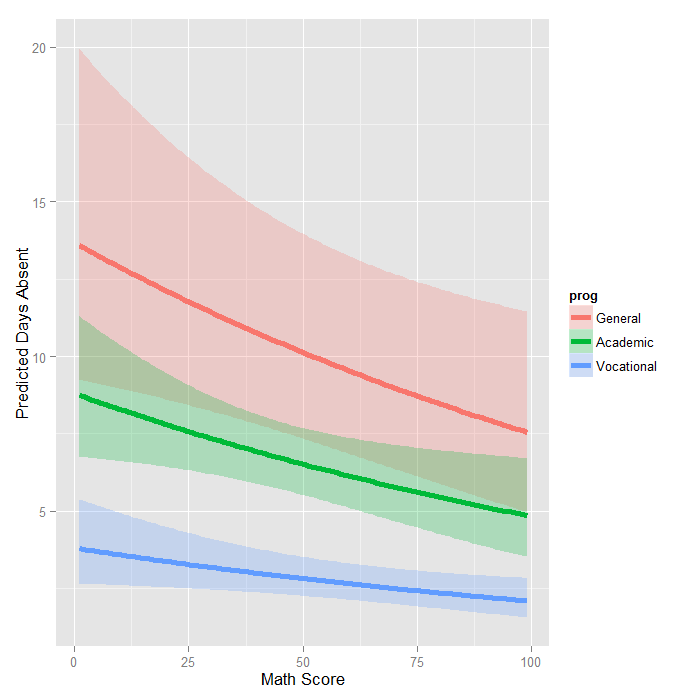
\includegraphics[width=0.7\linewidth]{negbin2}
\caption{}
\label{fig:negbin2}
\end{figure}
	
\end{frame}
	%================================================ %
	\begin{frame}[fragile]
		\frametitle{Negative Binomial Regression with \texttt{R} }
		\large
		
		\begin{framed}
			\begin{verbatim}
			
			ggplot(newdata2, aes(math, DaysAbsent)) +
			geom_ribbon(aes(ymin = LL, ymax = UL, fill = prog), alpha = .25) +
			geom_line(aes(colour = prog), size = 2) +
			labs(x = "Math Score", y = "Predicted Days Absent")
			
			\end{verbatim}	
		\end{framed}
		
\end{frame}
%================================================ %
\begin{frame}[fragile]
	\frametitle{Negative Binomial Regression with \texttt{R} }
	\Large
	
	% Plot of the model predicted days absent with confidence intervals
	The graph shows the expected count across the range of math scores, for each type of program along with 95 percent confidence intervals. Note that the lines are not straight because this is a log linear model, and what is plotted are the expected values, not the log of the expected values.
\end{frame}



%================================================ %
\begin{frame}[fragile]
	\frametitle{Negative Binomial Regression with \texttt{R} }
	\Large
	
	\textbf{Things to consider}
	\begin{itemize}
	\item It is not recommended that negative binomial models be applied to small samples.
	\item One common cause of over-dispersion is excess zeros by an additional data generating process. 
	\item In this situation, zero-inflated model should be considered.
	\end{itemize}
\end{frame}
%================================================ %
\begin{frame}[fragile]
	\frametitle{Negative Binomial Regression with \texttt{R} }
	\Large
\begin{itemize}
	\item	
	If the data generating process does not allow for any 0s (such as the number of days spent in the hospital), then a zero-truncated model may be more appropriate.
	\end{itemize}
\end{frame}
%================================================ %
\begin{frame}[fragile]
	\frametitle{Negative Binomial Regression with \texttt{R} }
	\Large
	\begin{itemize}
	\item
	Count data often have an exposure variable, which indicates the number of times the event could have happened. 
	\item This variable should be incorporated into your negative binomial regression model with the 
	use of the offset option. 
	%See the glm documentation for details.
	\end{itemize}
\end{frame}
%================================================ %
\begin{frame}[fragile]
	\frametitle{Negative Binomial Regression with \texttt{R} }
	\Large
		\begin{itemize}
	\item
	The outcome variable in a negative binomial regression cannot have negative numbers.
	\item You will need to use the \texttt{m1\$resid} command to obtain the residuals from our model to check 
	other assumptions of the negative binomial model 
	% (see Cameron and Trivedi (1998) and Dupont (2002) for more information).
	\end{itemize}
\end{frame}


%================================================== %	
\end{document}
